\documentclass[conference]{IEEEtran}
%\IEEEoverridecommandlockouts
% The preceding line is only needed to identify funding in the first footnote. If that is unneeded, please comment it out.
\usepackage{cite}
\usepackage{amsmath,amssymb,amsfonts}
\usepackage{algorithmic}
\usepackage{graphicx}
\usepackage{textcomp}
\usepackage{xcolor}
\def\BibTeX{{\rm B\kern-.05em{\sc i\kern-.025em b}\kern-.08em
    T\kern-.1667em\lower.7ex\hbox{E}\kern-.125emX}}
\begin{document}

%%%%%%%%%
%% Title
\title{Towards using the POWDER platform for RF propagation validation\\}


%%%%%%%%%
%% Author Headings
\author{\IEEEauthorblockN{Jose Monterroso}
\IEEEauthorblockA{\textit{School of Computing} \\
\textit{University of Utah}\\
Salt Lake City, USA \\
u1054133@utah.edu}
\and
\IEEEauthorblockN{Jacobus Van der Merwe}
\IEEEauthorblockA{\textit{School of Computing} \\
\textit{University of Utah}\\
Salt Lake City, USA \\
kobus@cs.utah.edu}
\and
\IEEEauthorblockN{Kirk Webb}
\IEEEauthorblockA{\textit{School of Computing} \\
\textit{University of Utah}\\
Salt Lake City, USA \\
kwebb@cs.utah.edu}
\and
\IEEEauthorblockN{Gary Wong}
\IEEEauthorblockA{\textit{School of Computing} \\
\textit{University of Utah}\\
Salt Lake City, USA \\
gtw@cs.utah.edu}
}

\maketitle




%%%%%%%%%
%% Abstract
\begin{abstract}
The need to find more efficient ways to share and use wireless spectrum
has resulted in renewed interest in radio frequency (RF) propagation modeling.
The open and programmable nature of the POWDER (Platform for Open Wireless Data-driven 
Experimental Research) mobile and wireless platform offers a unique
environment in which to test and validate RF propagation modeling approaches. 
In this paper we present our work illustrating how POWDER based RF measurements
can be performed, as a form of ``ground truth'', and compared with predicted
RF signal strength based on a propagation model. 
We make use
of the Shout RF measurement framework available on POWDER to perform
a series of RF measurements. We compare these measurements with predicted 
power levels using the open source RF Signal Propagation, Loss, And
Terrain (SPLAT!) analysis tool. 
We present our results and a brief
terrain analysis to provide real-world context for it. Our work is ``packaged'' 
as a POWDER profile to allow others to repeat our analysis and to serve
as a starting point for further RF measurement and propagation related research.
\end{abstract}


%%%%%%%%%
%% Index Terms
\begin{IEEEkeywords}
RF propagation, Network Measurement, Network testbed, RF modeling tools, SPLAT!, Shout
\end{IEEEkeywords}




%%%%%%%%%
%% Introduction
\section{Introduction}

Ever increasing demand for mobile and wireless services, combined with the
fact that wireless spectrum is essentially a fixed resource, has led to 
significant interest in innovative approaches to use and/or share spectrum.
In the U.S. signifiant initiatives in this domain include the recently
completed DARPA spectrum collaborative challenge~\cite{sc2}, dynamic spectrum
sharing in the 3.5~GHz citizen broadband radio service (CBRS) band~\cite{fcc_cbrs},
and more recently an NSF initiative to explore the feasibility of realizing national
radio dynamic zones (NRDZ)~\cite{nsf_nrdz}.

A key enabling component in many spectrum sharing approaches involves 
the development of accurate RF propagation models. 
The open and programmable nature of the POWDER (Platform for Open Wireless Data-driven Experimental Research) mobile and wireless platform, being developed and
deployed in Salt Lake City, Utah, offers a unique environment in which to test
and validate RF propagation models. 
POWDER enables user controlled RF transmission/reception and provide
tools and an experimental workflow system that simplifies wireless
experimentation and the creation of repeatable experimental artifacts.
In the context of validating RF propagation models, POWDER 
offers a wide range of wireless endpoints (i.e., rooftop nodes, static nodes at 
human height, nodes on campus shuttles and portable nodes),
deployed across varied topological terrain (i.e., including a hilly
campus environment, as well as a built-up urban-like setting).

Our work presented here illustrate how the POWDER platform can be used to test and validate
RF propagation models. We perform 
RF measurements to provide a form of “ground truth”, and compared that
with predicted RF signal strength based on RF propagation modeling.
We specifically make use of the Shout RF measurement framework available on POWDER to perform a number of RF measurements~\cite{b2} and use SPLAT!, an open source RF signal propagation, loss, and terrain analysis tool~\cite{b3}, for propagation modeling.
Shout enables orchestrated RF transmission and reception across the POWDER platform.
We use Shout to perform RF measurements in Band~7 ($\sim$2600~MHz), Band~42
($\sim$3500~MHz), and Band~43 ($\sim$3700~MHz). We make use of POWDER rooftop and
fixed-endpoint (human height) nodes for our measurements.
For propagation modeling SPLAT! is configured with the RF characteristics
associated with the POWDER radios (i.e., location, antenna height and gain, transmission
power etc.) and we use the point-to-point propagation model provided by the tool
for our analysis.

The contributions of this work are the following. We use the POWDER Shout framework to collect RF measurements on multiple bands. We use the SPLAT! tool to model corresponding RF path propagation and compare the results. We create a POWDER profile enabling other researchers to replicate both our RF measurements and propagation modeling and to serve as a starting point for future research efforts in this space.


%%%%%%%%%
%% Background
\section{Background}
Depending on the environment and placement of the transmitter and receiver, the path between the two can be line-of-sight (LOS)
or more complex depending on the obstacles between them. When transmitting the radio wave, losses are achieved under the 
influence of diffraction, reflection and scattering~\cite{b4}. Multipath propagation is fairly common in every type
of radio wave transmission. In fact, more commonly in nonline-of-sight (NLOS) but not limited to it, multipath still occurs were the
received radio waves arrive with time delays from different directions, and with different amplitudes. When these waves combine
at the receiver they can either usefully combine or interfere with one another and cause distortion or fade (loss). 

\subsection{Path Loss Models}
Loss on the propagation path between the transmitter and the receiving antennas can be defined as the ratio of the transmitted to 
received power. This loss is called path loss and represents the ratio expressed in decibels (dB) which is expressed according to 
the Free space model (in dB) and can be given by the ``Friis equation" as: 
\begin{equation}
P_r(dBm) = P_t(dBm) + G_t(dB) + G_r(dB) - L_p(dB)\label{eq1}
\end{equation}
where,
\begin{equation}
L_p(dB) = 20\log_{10}(\frac{4\pi d}{\lambda})\label{eq2}
\end{equation}

Here, $d$ is the path length while the wavelength $\lambda = c / f$, where $c=3*10^8$ meters per second is the speed of light. 
$f$ is the center frequency. The path loss is $L_p$ and is called the ``free space path loss". The terms $P_r(dBm)$, $P_t(dBm)$
describe the received power and the transmit power, respectively. $G_t(dB)$ and $G_r(dB)$ are gains (when they are positive, 
the received power increases.) And as distance increases, $L_p(dB)$ increases, which because of the negative sign, reduces 
the received power. Free space is useful for space communications systems, or radio astronomy. But not for cellular 
telephony~\cite{b5}.

However, we must take into account that obstructions exist in our real world and thus the free space model does not take into
account diffraction, and scattering losses~\cite{b5}. The path loss exponent model is a simple generalization of 
~\eqref{eq1} and ~\eqref{eq2} in which the exponent in the Friis model is allowed to change. We will see this in the results
section where we compare linear regression slopes of our acquired data. The path loss exponent model can be shown as:
\begin{equation}
P_r(dBm) = P_0(dBm) -10v\log_{10}(\frac{d}{d_0})\label{eq3}
\end{equation}
where $P_0 (dBm)$ is still given by the Friis equation,
\begin{equation}
P_0(dBm) = P_t(dBm) + G_t(dB) + G_r(dB) - 20\log_{10}(\frac{4\pi d_0}{\lambda})\label{eq4}
\end{equation}

Notice, that now the path loss after $d_0$ has changed to include a factor of $10v$ instead of 20. This is due to the nature of
the path loss exponent model where $v$ is defined to be the path loss exponent. $v$ is determined by empirical measurements
for the area in which the receiver and transmitter reside. The value of $v$ will be higher in dense cities, in buildings with highly
attenuating walls, in varying terrain, and when antennas are closer to the ground~\cite{b5}. 

\begin{figure}[htbp]
\centerline{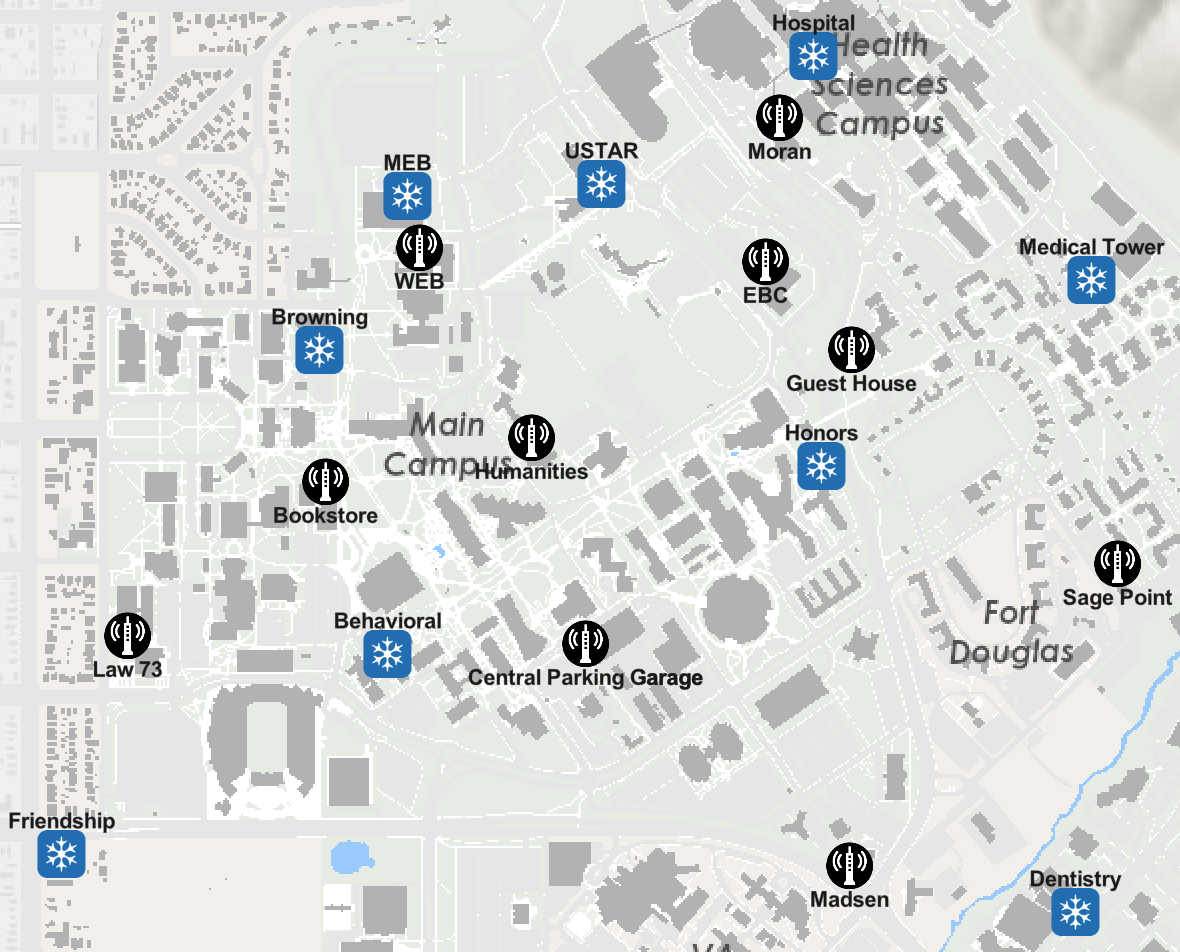
\includegraphics[width=0.8\columnwidth]{figs/currPowder.png}}
\caption{POWDER map showing current deployment. Snowflakes represent base stations. Black circles represent fixed endpoint nodes~\cite{b1}.}
\label{powdernodes}
\vspace{-3mm}
\end{figure}

\subsection{Propagation Models}
A propagation model is a tool that is important in the process of planning, developing and analyzing of radio communication 
networks. There is not a one size fits all type of approach when it comes to propagation models. The use of particular 
propagation models depends on the parameters available for the chosen area of the propagation study as well as the 
different parameters of the model. Propagation models can be categorized into two common groups: empirical and 
deterministic models. Deterministic models are based on the physical laws of wave propagation to determine the received 
signal power and often require a detailed map of the propagation environment. Empirical models are based on observations 
and measurements alone and are mainly used to predict path loss.

There is a vast array of propagation models including: Longley-Rice, Okumura-Hata, COST-231, Egli, and others. From the ones 
listed Longley-Rice is by far the most widely known and used. In fact, our modeling tool SPLAT! is based on the Longley-Rice 
model~\cite{b6}. The Longley-Rice model is based on electromagnetic theory and on statistical analysis of both 
terrain features and radio measurements. The model can act as an area prediction model or as a point-to-point model. To use
the model, one computes the additional loss to each path obstruction. These losses are summed and then added to the 
predicted line of sight path loss which is calculated using the Friis transmission equation in SPLAT!.

\subsection{Unknown Reference}
In the current POWDER deployment, radios are uncalibrated~\footnote{Efforts are currently underway to calibrate all POWDER radios to remedy this shortcoming.}. This means that when we take power measurements, we will have
power values with respect to an unknown reference~\cite{b5}. The receiver still provides a dB measurement 
of power, however, there is no known reference. 
This provides a challenge when comparing data/measurements as you cannot compare point-to-point values. 

Ultimately the solution involves calibrating the RF receivers and transmitters.  In our evaluation we follow an alternative approach involving a relative comparison of the
path loss exponent from equation~\ref{eq3}.



%%%%%%%%%
%% Measurement Methodology 
\section{Measurement Methodology}
\label{sec:method}
Our measurements are conducted on the current POWDER deployment
on the University of Utah campus (Fig.~\ref{powdernodes}).
Part of the area includes a typical spread out university campus, while other parts
include a more densely populated urban-like environment. POWDER offers nine general purpose rooftop base stations that include networked software-defined-radios (SDRs), an RF front-end (frequency division duplex), and signal amplification. Furthermore, POWDER offers 10 fixed endpoints. 
Similar to the general purpose rooftop base stations, the components include SDRs, RF front-end and antenna elements. 

\subsection{Measurement Tool: Shout}
Shout is a measurements framework developed by the POWDER team~\cite{b2}. Using Shout you are able to collect RF
measurements for the nodes within the testbed. The framework was developed in Python and offers a rich set of measurement
collections. Shout follows a client-server architecture in which we have an orchestrator node running at all times. Each client 
radio node connects to the orchestrator via the POWDER control/out-of-band network. 

For our purposes we used Shout to collect RF propagation among the nodes on the platform. Shout uses JSON files as 
command files to tell the orchestrator how it should direct the other nodes. We used a configuration file which directed the
framework to treat each node as a receiver and transmitter in a round-robin fashion. The JSON file used follows this approach:
\begin{equation}
PL_M = CF + \frac{1}{2}SR\label{eq5}
\end{equation}
Where $CF$ is the center frequency (tuned frequency) and $SR$ is the sample rate. $PL_M$ describes the upper bound for
collection, with a frequency step size dictated by the JSON file. In other words for the given $CF$ we collect measurements 
up to $PL_M$ with a given frequency step. Shout then averages these results to produce an average received power for the
given frequency between two nodes. This is the approach we follow when calculating RF propagation using the Shout framework.

\subsection{Measurement Tool: SPLAT!}
SPLAT! will be our modeling tool to compare with Shout's results~\cite{b3}. SPLAT! can be used to produce terrain analysis 
maps of the designated area, but for our purposes we will use the SPLAT! point-to-point analysis model to calculate RF 
propagation. For RF propagation, SPLAT! requires two primary files: QTH, and LRP. QTH files are site location files that contain
the site's name, the site's latitude, the site's longitude and the site's antenna height above ground level. LRP files are the irregular
terrain model parameter files that are used to determine radio frequency path loss, field strength, or received signal power level. 

\begin{figure}[htbp]
\centerline{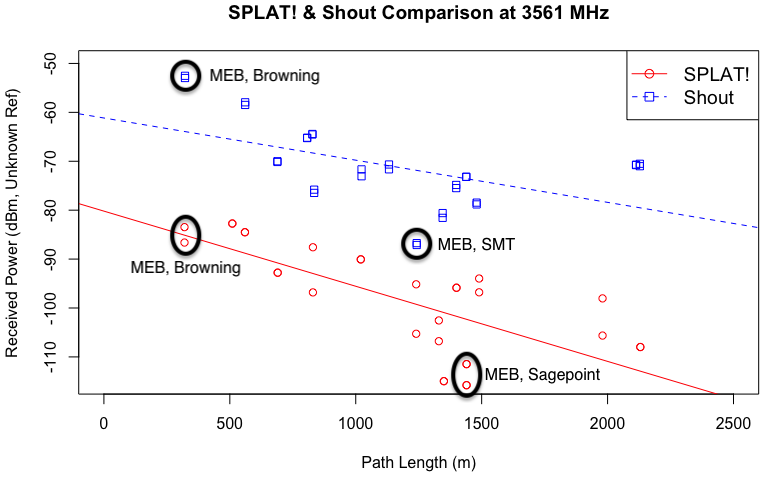
\includegraphics[width=0.9\columnwidth]{figs/3561.png}}
\vspace{-3mm}
\caption{Run 1. Used 3561 MHz frequency.}
\label{3561}
\vspace{-3mm}
\end{figure}

\begin{table}[htbp]
\caption{Path Loss Exponents for each run}
\begin{center}
\begin{tabular}{|c|c|c|c|}
\hline
\textbf{Run \#} & \textbf{\textit{Frequency (MHz)}}& \textbf{\textit{Shout (dBm/m)}}& \textbf{\textit{SPLAT! (dBm/m)}} \\
\hline
Run 1& $3561$& $-0.0086$& $-0.0154$  \\
Run 2& $2620$& $-0.0114$& $-0.0186$  \\
Run 3& $3550$& $-0.0132$& $-0.0113$  \\
Run 4& $3690$& $-0.0163$& $-0.0103$  \\
\hline
\end{tabular}
\label{tab1}
\vspace{-3mm}
\end{center}
\end{table}

To produce and compare accurate results between Shout and SPLAT!, we followed the same approach as in formula \eqref{eq5}. Using the 
proper QTH and LRP files for each node we created a Python script that easily mediates the process of collecting the data
for a given frequency. SPLAT! is a command-line driven application that reads in the data from the QTH and LRP files and produces a 
results file that can be parsed for the necessary data. 


\subsection{Measurements}
Following the above methodology we perform extensive measurements on the POWDER platform using Shout and SPLAT! using
multiple frequencies and nodes. For this effort we conducted four measurement runs with each run being done three times. These measurement runs span three different frequency ranges. To summarize: 
\begin{itemize}
\item Run 1 took place in early October. The measurement conducted used the 3561 MHz frequency, and used the: Behavioral 
Science, Browning, Friendship Manor, Sagepoint, MEB, and South Medical Tower nodes. This run was conducted at mid-day. 
\item Run 2 took place in early November. The measurement conducted used the 2620 MHz frequency, and used the: Behavioral
Science, Browning, Friendship Manor, Honors, Sagepoint, Ustar as transmitters nodes. And used Bookstore, EBC, Garage, 
Guesthouse, Humanities, Law73, Madsen, Moran, and WEB as receiver fixed endpoint nodes. This run does not follow the 
typical round-robin approach among all the nodes where each one acts as a receiver and transmitter because only the transmitter
nodes listed where able to transmit at the listed frequency. We still followed the approach discussed in equation~\eqref{eq5}.  This run was
conducted early morning. 
\item Run 3 took place in late November. The measurement conducted used the 3550 MHz frequency, and used the: Behavioral
Science, Browning, Honors, Sagepoint, South 

\begin{figure}[htbp]
\centerline{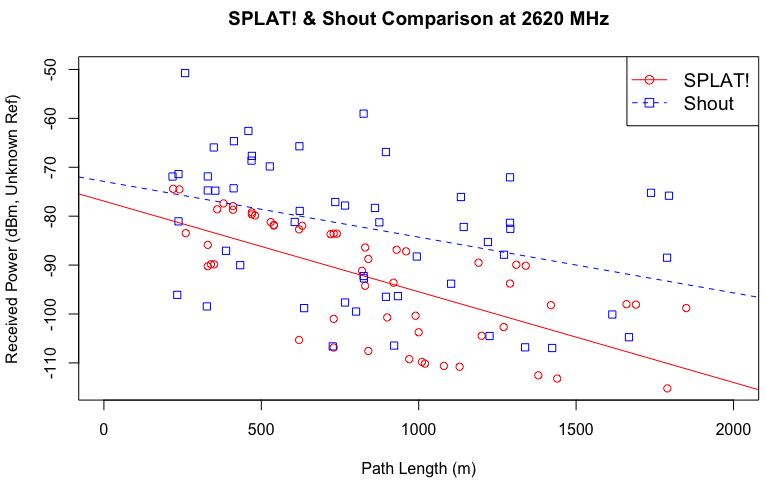
\includegraphics[width=0.9\columnwidth]{figs/2620.png}}
\vspace{-3mm}
\caption{Run 2. Used 2620 MHz frequency.}
\label{2620}
\vspace{-3mm}
\end{figure}

Medical Tower, Ustar, and Friendship Manor nodes. This run was conducted early 
morning. 
\item Run 4 took place in late November. The measurement conducted used the 3690 MHz frequency, and used the: Behavioral 
Science, Browning, Honors, Sagepoint, South Medical Tower, Ustar, and Friendship Manor nodes. This run was conducted early 
morning.
\end{itemize}




%%%%%%%%%
%% Results and Discussion
\section{Results and Discussion}
After the four measurement runs completed on Shout, we perform an analysis with the SPLAT! tool using the same frequencies, 
radio locations and following the same method discussed in Section~\ref{sec:method}.
We convert our acquired data into plots through the use of our python script. 
Each dot on the plot is a pairwise connection between the transmitter
and receiver at the given frequency. Due to the multitude of dots we refrain from naming each dot as it overwhelms the plot. Due to the unknown reference for either Shout or SPLAT! we are unable to directly compare the two.
However, we will compare the two using the path loss exponent which happens to be the slope of the linear regression line of transmission power versus distance plot. 
Following the path loss exponent analysis we will do a brief terrain analysis of the results we obtained. 

\subsection{Path Loss Exponent}
Due to the POWDER platforms uncalibrated radios there is not a single reference point for the Shout data. This is the reason 
why all of our plots for each run define the Y-axis as the received power in dBm with an unknown reference. Notice that SPLAT!'s
data is represented by the red color while Shout's data is represented by the blue color. Table~\ref{tab1} summarizes the path 
loss exponents for each run.

Run 1 (Fig.~\ref{3561}), was conducted on the 3561 MHz frequency in early October 2020 at around 11AM. This run followed
the typical round-robin fashion, where each circle on the plot represents a pairwise connection between the transmitter and receiver. 
The slope for Shout in run 1 was $-0.00862$, this tells us that the power decays proportionally to $d^{-0.00862}$ where $d$ is the 
path length. Similarly, we determined the measurements fit of SPLAT!. The path loss exponent is $-0.0154$ that is the power decays 
proportionally to $d^{-0.0154}$. We can see SPLAT!'s path loss exponent has a steeper slope. That is for the 3561 
\begin{figure}[htbp]
\centerline{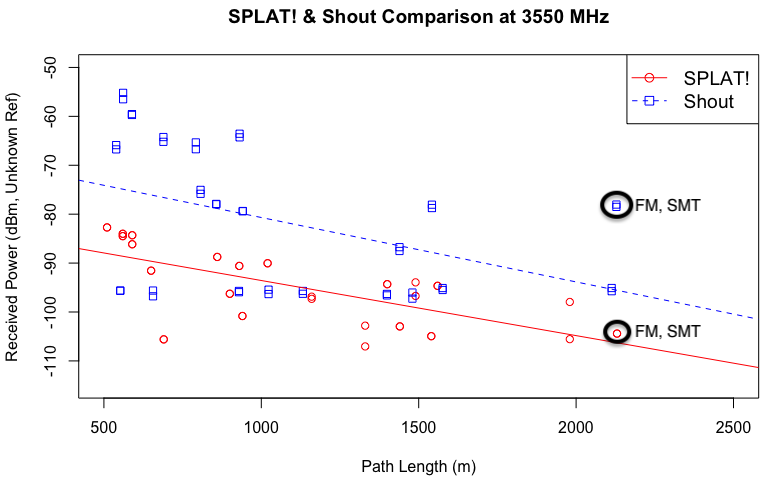
\includegraphics[width=0.9\columnwidth]{figs/3550.png}}
\vspace{-3mm}
\caption{Run 3. Used 3550 MHz frequency.}
\label{3550}
\vspace{-3mm}
\end{figure}
\begin{table}[htbp]
\caption{Run 1, best path loss for Shout and SPLAT!}
\begin{center}
\begin{tabular}{|c|c|c|}
\hline
\textbf{Data Set} & \textbf{\textit{Nodes}}& \textbf{\textit{Received Power (dBm)}} \\
\hline
Shout& MEB, Browning& $-52$ \\
SPLAT!& MEB, Browning& $-83$ \\
\hline
\end{tabular}
\vspace{-3mm}
\label{tab2}
\end{center}
\end{table}
MHz frequency, SPLAT! has over-predicted the path loss when compared to Shout's ground truth measurements. 

We now conduct a similar procedure for the remaining runs. Run 2 (Fig.~\ref{2620}) was conducted in early November 2020 at
around 9AM and used the largest amount of nodes within our experiments. Shout's path loss exponent was $-0.0114$ with a power 
decay proportional to $d^{-0.0114}$. While SPLAT!'s path loss exponent was $-0.0186$ with a power decay proportional to 
$d^{-0.0186}$. These are fairly close but once again SPLAT! is over-predicting the POWDER platform's radio path loss at the 2620 
MHz frequency. 

Run 3 (Fig.~\ref{3550}) and run 4 (Fig.~\ref{3690}) were conducted in late November 2020. Specifically, run 3 was 
conducted at around 2AM while run 4 occurred around 6AM. For run 3, Shout's path loss exponent is $-0.0132$ while SPLAT!'s 
is $-0.0113$. Run 3 offers the closest in comparing the path loss exponent values for the data collected. However, this time SPLAT! 
is under-predicting the POWDER platforms path loss for the 3550 MHz frequency. Similarly, in run 4 we see SPLAT! under-predicting
the path loss on the 3690 MHz frequency. In run 4 we see that Shout's path loss exponent is $-0.0163$, while SPLAT!'s path loss 
exponent is $-0.0103$. 

\subsection{Terrain Analysis}
The purpose of this section is to bring SPLAT! to real life and compare the model to physical locations. We utilize Google 
Maps to take a closer view of the environment in run 1. Notice that in Fig.~\ref{3561}, we label the best and worst path loss 
nodes for each data set. We will focus on the two nodes with the best path loss, and the two nodes with the worst path loss and 
compare Shout and SPLAT! when differences arise. 

\subsubsection{Best Path Loss}
We first look at the two nodes in run 1 with the best path loss. Table~\ref{tab2} lists the best path loss nodes for both Shout and 
SPLAT!, at the 3561~MHz frequency. We can see that for both data sets, MEB and Browning hold the best propagation values. 
Fig.~\ref{mebBrown} shows the Google Maps
\begin{figure}[htbp]
\centerline{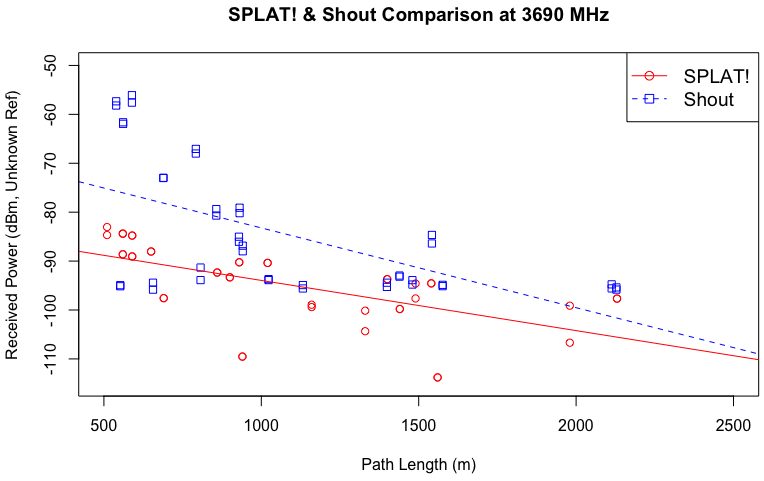
\includegraphics[width=0.9\columnwidth]{figs/3690.png}}
\vspace{-3mm}
\caption{Run 4. Used 3690 MHz frequency.}
\label{3690}
\vspace{-3mm}
\end{figure}
\begin{table}[htbp]
\caption{Run 1, worst path loss for Shout and SPLAT!}
\begin{center}
\begin{tabular}{|c|c|c|}
\hline
\textbf{Data Set} & \textbf{\textit{Nodes}}& \textbf{\textit{Received Power (dBm)}} \\
\hline
Shout& MEB, SMT& $-87$ \\
SPLAT!& MEB, Sagepoint& $-115$ \\
\hline
\end{tabular}
\label{tab3}
\vspace{-3mm}
\end{center}
\end{table}
image of the two nodes. Both nodes are rooftop base stations with LOS. We believe that these two nodes received the
best propagation simply due to the distance between them and the fact that there is 
nothing directly blocking them.  

\subsubsection{Worst Path Loss}
We now look at the two worst nodes with regards to propagation loss. Table~\ref{tab3} lists the worst path loss nodes for both 
Shout and SPLAT! at the 3561~MHz frequency. For SPLAT! these two nodes are MEB and Sagepoint. We note that Sagepoint 
is the only fixed endpoint node for run 1 and is 1.5~meters above the ground, while MEB is a rooftop base station. From 
Fig.~\ref{worst} we notice that the environment between MEB and Sagepoint is NLOS. In fact, three sports fields, the student
life center, a busy road, and multiple housing units lie in-between these two nodes. Furthermore, since Sagepoint is a 
fixed endpoint node it is placed behind a wall that is not facing the MEB. 

However, Shout thinks differently. It believes that the two worst nodes are MEB, and South Medical Tower (SMT). The environment
between these two include the Biotechnology Building, a busy road, parking structures, and the College of Pharmacy.
However, both MEB and SMT are rooftop base stations with MEB being the shorter one. 

\subsection{Discussion}
We now offer a few insights as to why we got the results we did. We can see how early hours affected Shout's data in run 3. 
In Fig.~\ref{3550} where we can see that at a striking distance of about 2128 meters we appear to be getting $-78$ dBm 
in received power compared to SPLAT!'s $-104$ dBm, for the Friendship Manor and SMT nodes. Again we can't compare 
point-to-point due to unknown reference, but this appears to be an outlier
when compared to the rest of Shout's data where 
about half the points are underneath $-78$ dBm given their respective smaller path length.

\begin{figure}[htbp]
\centerline{\includegraphics[width=0.9\columnwidth]{figs/mebBrown.png}}
\caption{MEB left and Browning right.}
\label{mebBrown}
\vspace{-3mm}
\end{figure}

\begin{figure}[htbp]
\centerline{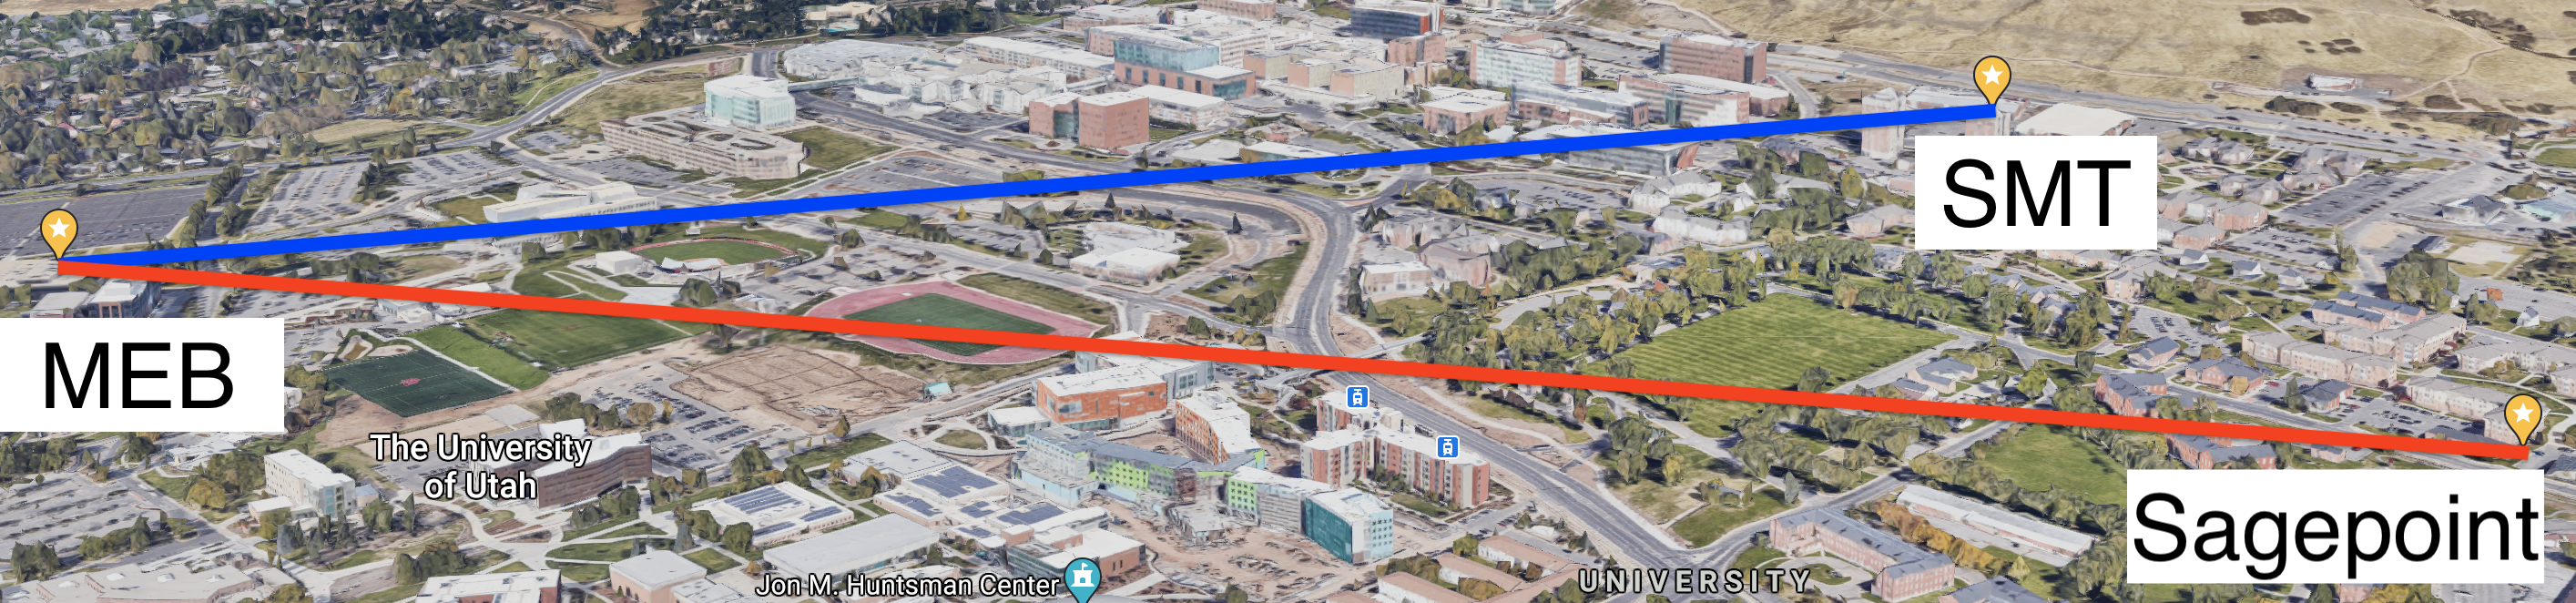
\includegraphics[width=0.9\columnwidth]{figs/worst.png}}
\caption{SPLAT! (Red): MEB to Sagepoint; Shout (Blue): MEB to SMT.}
\label{worst}
\vspace{-3mm}
\end{figure}

As expected for all cases in every run we saw power levels with exponentially decreasing magnitude as a function of 
distance. Meaning that in all cases we saw propagation loss increase with distance. As discussed in the background section, 
there exists multiple path loss models that can be used depending on the parameters available to us. For example, SPLAT! 
follows the Longley-Rice path loss model, and this model might not be sophisticated
enough to accomodate the topology found in our experiment.

Note that our goal with this work is not to evaluate the accuracy of the SPLAT! tool
per se, but rather to illustrate the utility of the POWDER platform to conduct research 
of this nature. Specifically, the ability to perform longitudinal studies on POWDER, spanning different weather conditions and seasons, coupled with the flexibility
and rich diversity of the platform, suggests the usefulness of POWDER for this type of
research.   


%%%%%%%%%
%% Related Works
\section{Related Work}
The idea of measuring RF propagation~\cite{b8, b9} as well as using propagation models to
predict RF propagation loss~\cite{b4, b10} is not a new idea. We first cover related
work associated with comparisons of the accuracy of different propagation models.
We then consider related efforts that specifically used the SPLAT! tool used in our work
and then consider related work what used the CloudRF radio propagation modeling tool. 

\subsection{Propagation Models}
A comparison of three path loss models for fixed wireless access systems was done~\cite{b16}. The comparison
measurements were taken at 3.5 GHz in Cambridge, UK and their applicability was validated in three environments: rural, suburban,
and urban environments. Specifically, three empirical models the Stanford University Interim (SUI), the COST-231 Hata, and the ECC-33 
models were chosen for this comparison. The results show that ECC-33 model shows the best results, especially in urban environments.
While for the general case the COST-231 Hata and SUI models highly over predict the path loss in all the environments.

\subsection{SPLAT!}
SPLAT! is one of few open source RF propagation modeling analysis tools~\cite{b3}. 
SPLAT! allows for propagation loss and terrain analysis for the electromagnetic spectrum between 20 MHz and 20 GHz. Our first 
example of SPLAT! is used in an architecture that can be used for simulation and in-situ learning of the attenuation
of RF signals in the environment~\cite{b12}. In this earlier work SPLAT! is used to generate a prediction mean field for CU Mountain Research Station to determine
radio frequency propagation loss in the rocky terrain. 

Another study, that resembles ours, aims to compare accurate measurements taken by Rohde \& 
Schwarz portable spectrum analyzer and precision antennas for digital TV, with simulated results from multiple coverage prediction 
models like SPLAT!~\cite{b6}. However, SPLAT! in this study produces big differences compared with the real measurement results. This is 
due to SPLAT!'s inability to work properly in the LOS mode as well as a lack of detailed terrain information. 

Digital Terrestrial Television (DTT) is degraded due to the coexistence between LTE operating in the adjacent
frequency band~\cite{b13}. To study these results the authors of this earlier effort used SPLAT! to produce a DTT system model. To produce such a 
model they took into account earth conductivity, atmospheric bending constant, antenna polarization, relative permittivity, and 
antenna height above the ground.

\subsection{CloudRF}
CloudRF
is another radio propagation modeling tool that offers more in terms of cellular propagation models for mobile networks, 
as well as faster results due to its proprietary propagation engine~\cite{b11}. 
Long Range (LoRa) is a low-power wide-area networking protocol that is designed to connect Internet of Things (IoT) devices to the 
internet in regional, national or global networks. Deployment of LoRa access points requires taking into consideration the spatial 
distribution of clients, and radio signal propagation. A heuristic algorithm was designed for gateway location
selection for LoRa networks~\cite{b14}. In this earlier effort CloudRF was used to estimate the coverage of LoRa gateways on the map allowing the algorithm to
decide if the placement of access nodes are at the best place they could be. 

Similarly, a simulation was done to replace the Peruvian Navy's Supervisory Control and Data Acquisition (SCADA) 
system with an IoT-based solution using LoRaWAN~\cite{b15}. SCADA is a system to monitor and control remote meteorological and luminous 
stations. Path loss calculations between stations were made using the Okumura-Hata radio propagation model. The results were then 
validated using CloudRF. Results conclude that the LoRaWAN system is superior to the currently used SCADA system. 



%\fi
%%%%%%%%%
%% Conclusion
\section{Conclusion}

In this paper we present our work on using the POWDER mobile and wireless
research platform to conduct RF propagation related research. We showed
how ground truth RF measurements obtained from the POWDER platform can
be compared with an RF propagation prediction tool. 
Specifically, we performed measurements using the Shout measurement framework
and compared the resulting data with predicted power levels obtained from the
SPLAT! RF propagation tool. 

While useful in its own right to inform our efforts as we continue 
to build out the POWDER platform, the primary aim of our work is to
illustrate the utility of POWDER to enable this type of research. To that end,
we have packaged our work into a POWDER profile that enables others to
replicate our results and to serve as a starting point for related research
efforts~\cite{paper_profile}. 

\iffalse
In this paper we discussed RF propagation. Specifically, we covered RF propagation models, ran a few measurements on the 
POWDER platform, discussed our results, and compared the data between our propagation model and the ``ground truth". 
SPLAT! was our RF propagation model of choice and its measurement results were compared with the Shout framework. Shout 
was developed by the POWDER team to conduct measurement studies on the POWDER platform. 

Our results showed that SPLAT! on the 3561 MHz and 2620 MHz frequencies overpredicted the path loss, however on the 3550 
MHz and 3690 MHz SPLAT! under-predicted the path loss with respect to the Shout framework. Furthermore, on the 3561 MHz
frequency, Shout and SPLAT! both picked the same two nodes with the best RF propagation, but failed to choose the same two 
nodes when it came to picking nodes with the worst RF propagation. There is no definitive answer as to whether or not Shout 
has been validated with respect to SPLAT!. RF propagation models take into account multiple parameters to calculate path loss,
it could just so be that SPLAT! is not the ideal model for the POWDER platform.
\fi



%%%%%%%%%
%% References
\bibliographystyle{bibtex/IEEEtran}
\bibliography{bibtex/IEEEabrv,bibtex/bibliography}

\end{document}
